%%%%%%%%%%%%%%%%%%%%%%%%%%%%%%%%%%%%%%%%%%%%%%
%                insertmeeting
% 1) Title (something creative & funny?)
% 2) Date (MM/DD/YYYY)
% 3) Location (ex. Hagerty High School)
% 4) People/Committees Present 
% 5) Picture 
% 6) Start Time & Stop Time (ex. 12:30AM to 4:30PM)
%%%%%%%%%%%%%%%%%%%%%%%%%%%%%%%%%%%%%%%%%%%%%%
\insertmeeting 
	{Can't Make Any Promises} 
	{03/31/22} 
	{Hagerty High School}
	{James, Jensen, Nathan, Ritam}
	{Images/RobotPics/robot.jpg}
	{2:30 - 4:30}
	
\hhscommittee{Software}
\noindent\hfil\rule{\textwidth}{.4pt}\hfil
\subsubsection*{Goals}
\begin{itemize}
    \item Try out an arm brake mode.

\end{itemize} 

\noindent\hfil\rule{\textwidth}{.4pt}\hfil

\subsubsection*{Accomplishments}
One thing we did not realize earlier was that we can change the braking behavior of the arm. In this case, we did not have a brake mode set. We decided to try using "intakeMotor.setZeroPowerBehavior(DcMotor.ZeroPowerBehavior.BRAKE);" in our code to stop the motor when it reaches the target position. This might allow us to move the arm at much higher speeds, then braking it before we begin the positional PID we talked about a few weeks ago. However, upon testing, we weren't able to find a satisfactory solution to the problem. Because this issue is less urgent than fine-tuning the autonomous program, we'll put it on the shelf until we have some more free time. 


\begin{figure}[htp]
\centering
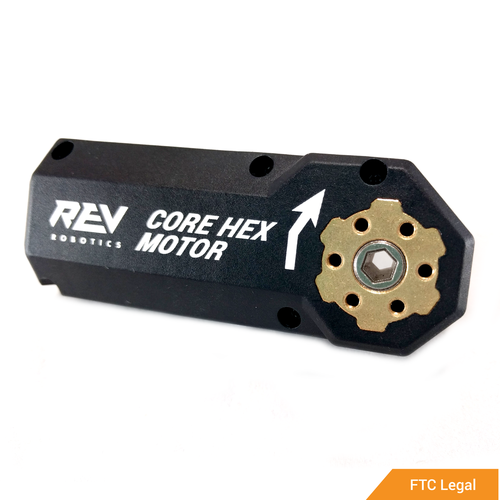
\includegraphics[width=0.95\textwidth, angle=0]{Meetings/March/03-31-22/03-31-22 1.jpg}
\caption{A REV Core Hex Motor that we were adjusting the brake behavior on.}
\label{fig:033122_1}
\end{figure}



\whatsnext{
\begin{itemize}
    \item Continue improving autonomous.
\end{itemize} 
}

